\documentclass{beamer}

\mode<presentation>
{
  \usetheme{Madrid}      % or try Darmstadt, Madrid, Warsaw, ...
  \setbeamertemplate{navigation symbols}{}
  \setbeamertemplate{caption}[numbered]
} 

\colorlet{beamer@blendedblue}{black}

\usepackage[french]{babel}
\usepackage[utf8x]{inputenc}
\usepackage[T1]{fontenc}
%\usepackage[squaren,cdot]{SIunits}
\usepackage{graphicx}
\usepackage{listings}

\graphicspath{}

\logo{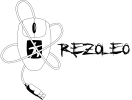
\includegraphics[height=0.8cm]{rezoleo.png}\vspace{10pt}\hspace{20pt}}
\title{Couche transport}
\author{LEDER "Ziman" Simon}
\institute{Rezoleo\\}
\date{\today}

\begin{document}
	
	\begin{frame}
		\titlepage
	\end{frame}

\section{Problematique}
	
	\begin{frame}{Problématique}
		\begin{itemize}
			\item[\textbullet] L'ordre des paquets ?
			\item[\textbullet] Quid des paquets perdus ?
			\item[\textbullet] Comment gérer plusieurs applications ?
			\item[\textbullet] Que faire si une application prend toute la bande passante ?
		\end{itemize}
	\end{frame}

\section{Role}

	\begin{frame}{Rôle}
		\begin{itemize}
			\item[\textbullet] Etablissemnt d'une communication entre deux applications
			\item[\textbullet] Suivi des conversations individuelles 
			\item[\textbullet] Segmentation des données et reconstitution des segments
			\item[\textbullet] Identification des applications
		\end{itemize}
	\end{frame}

	\begin{frame}{Suivi des connexions individuel}
		\textbf{Converstation} : l'ensemble des données qui transit entre 2 applicatons \\
		Une machine sur le réseau peut héberger plusieurs applications qui conversent avec plusieurs autres applications\\
		La couche transport est chargée de garantir ces multiples conversations et d'en effectuer le suivi.
	\end{frame}


	\begin{frame}{Découpage des données}
		La plupart des réseaux limite la longueur maximale des paquets qui y transitent. C'est le rôle de la couche transport de découper les données.\\
		La couche transport ajoute au paquet un en-tête permettant la reconstitution et la réorganisation des paquets. C'est la {\textbf segmentation}\\
	\end{frame}

	\begin{frame}{Multiplexage}
		Que faire si une application utilise toute la bande passante ? \\
		La couche transport est chargée de permettre à plusieurs application de communiquer en même temps. La segmentation permet à plusieurs éléments d'être imbriquer dans le flux.
	\end{frame}

	\begin{frame}{Découpage des données}
		\begin{figure}
			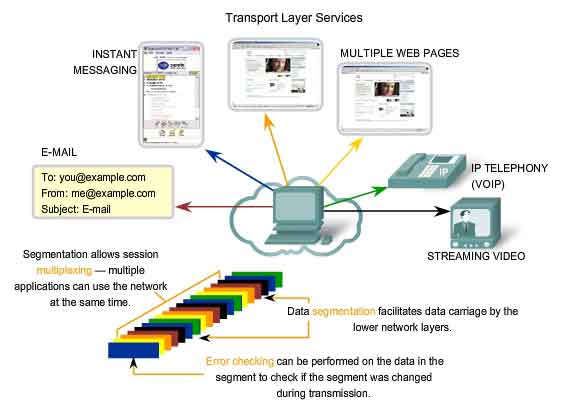
\includegraphics[scale=0.4]{TRANSPORT.jpg}
		\end{figure}
	\end{frame}

	\begin{frame}{Fiabilité}
		Les applications ont une certaine exigence de fiabilité\\
		La couche transport possède deux protocoles pour gérer la fiabilité du transport des paquets : TCP et UDP.
		\begin{figure}
			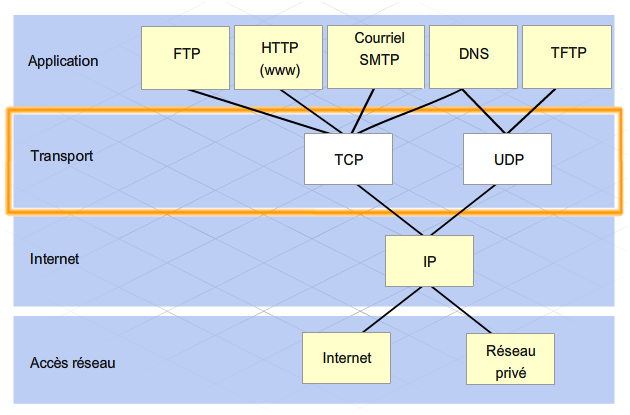
\includegraphics[scale=0.5]{UDP.png}
		\end{figure}
	\end{frame}

\section{TCP vs UDP}

	\begin{frame}{TCP}
		\textbf{TCP} : Transport Communication Protocol
		3 fonctions de fiabilité : 
		\begin{itemize}
			\item[\textbullet] Numérotation et suivi des segments de données transmis à un hôte donné à partir d'une application spécifique
			\item[\textbullet] Accusé de réception des données reçues
			\item[\textbullet] Retransmission des données pour lesquelles aucun accusé de réception n'a été reçu, après un certain temps
		\end{itemize}
	\end{frame}

	\begin{frame}{TCP}
		\begin{figure}
			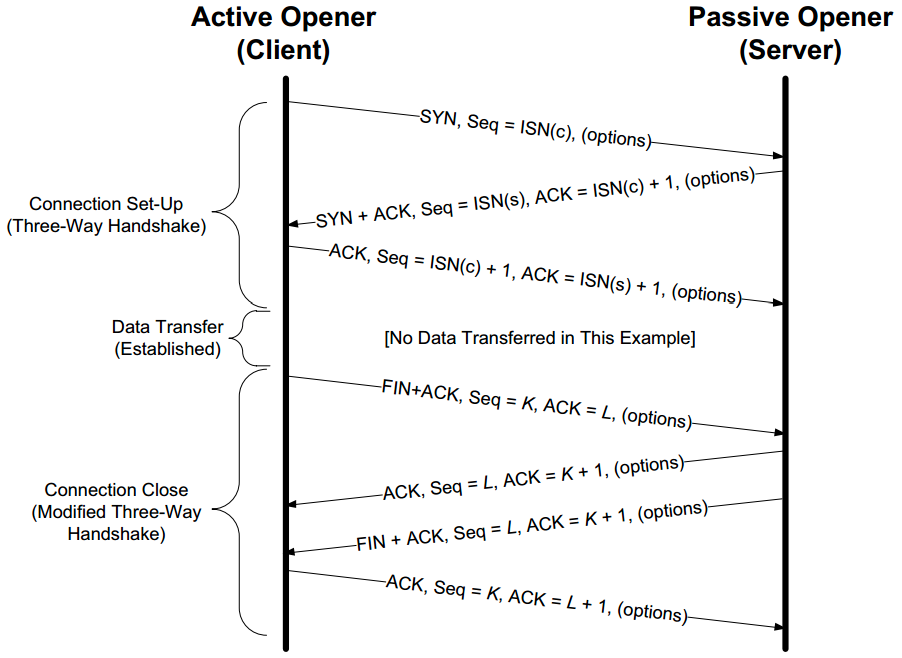
\includegraphics[scale=0.3	]{TCP.png}
		\end{figure}
	\end{frame}	

	\begin{frame}{TCP}
		\begin{figure}
			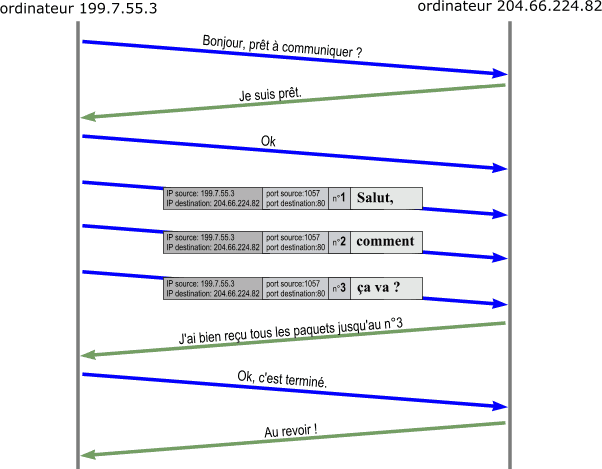
\includegraphics[scale=0.4]{TCPSimple.png}
		\end{figure}
	\end{frame}

	\begin{frame}{UDP}
		\begin{figure}
			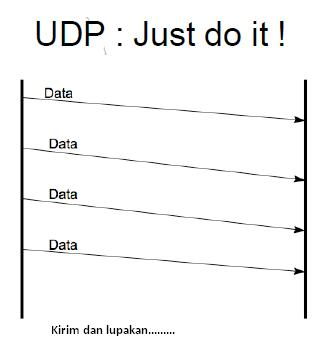
\includegraphics[scale=0.6]{udpsimple.jpg}
		\end{figure}
	\end{frame}

\section{Les ports}

	\begin{frame}{Les ports}{Le problème}
	\begin{figure}
		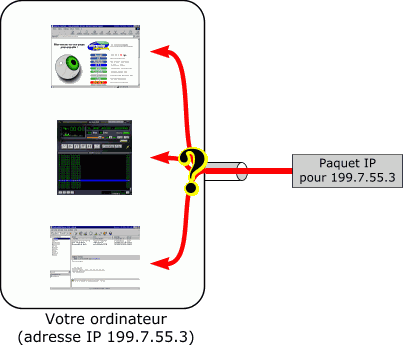
\includegraphics[scale=0.4]{port1.png} \hspace{0.5cm}
		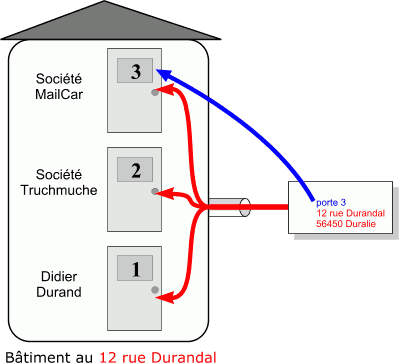
\includegraphics[scale=0.4]{port2.png}
	\end{figure}
	\end{frame}	
	\begin{frame}{Les ports}
		\begin{center}
		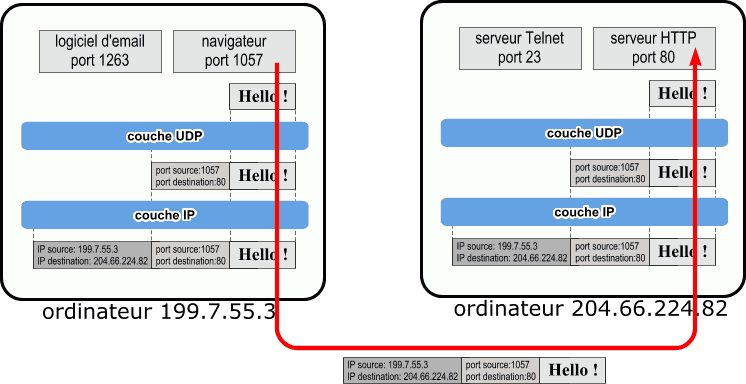
\includegraphics[scale=0.4]{port4.png}
		\end{center}
	\end{frame}

	\begin{frame}{Les well-known ports}
		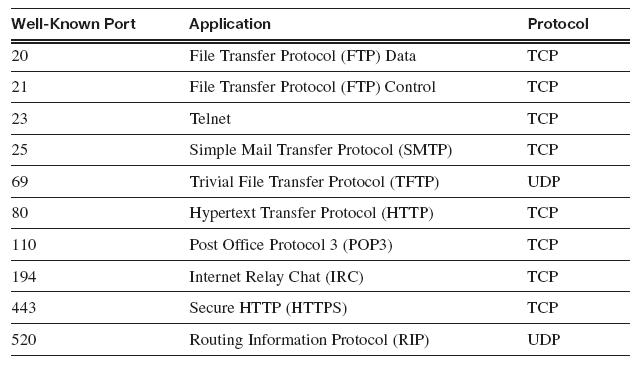
\includegraphics[scale=0.7]{wkports.jpg}
	\end{frame}
\end{document}